\section{Opzet van het model}
We hebben ons systeem ingedeeld in de volgende onderdelen:
\begin{itemize}
    \item Lamp (UV en/of LED)
    \item Sensor
    \item Lopende Band (vooruit)
    \item Lopende Band (voor- en achteruit)
    \item Startknop
    \item Noodknop
    \item Deur
    \item FallOff**
    \item Luchtklep*
    \item Compressor*
    \item Pneumatische Cilinder*
    \item Bak (gelukt en afval)

\end{itemize}

De onderdelen gevolgd door ** kunnen niet in het hardware model worden opgenomen, dit zijn geen fysieke componenten. \\
De onderdelen gevolgd door * zijn niet opgenomen in het UPPAAL model. Onder andere omdat ze altijd aan moeten zijn, of door een ander onderdeel, dat w\'el gemodelleerd is, bestuurd worden. \\ \\

Hieronder bespreken wij alle onderdelen aan de hand van foto's van ons model. Hierbij hebben wij gebruik gemaakt van foto's waarbij, na omcirkeling, een onderdeel nog herkenbaar is. \\ \\

Wegens de conversie door \LaTeX bij het invoeren van plaatjes met transparency, zijn er zwarte vlakken om onze foto's ontstaan. Onze excuses voor eventuele ongemak.


\section{Foto's van het model}\label{sec:foto_s_van_het_model} % (fold)

\subsection{Lamp}\label{sub:Lamp} % (fold)


  
\includegraphics[width=13cm, height=11cm]{lamp} \\
  \includegraphics[width=13cm, height=8cm]{UVlamp} \\

Op deze foto's zijn de eerste LED respectievelijk de UV-lamp te zien.
De tweede LED kan niet worden gefotografeerd wegens obstructies. \\
Tegenover de twee LED's staat bij ieder \'e\'en sensor, deze worden hierna behandeld.


% subsection lamp (end)

\subsection{Sensor}\label{sub:sensor} % (fold)
  
\includegraphics[width=13cm, height=14cm]{lamp} \\
  \includegraphics[width=13cm, height=9cm]{UVlamp} \\
  Op de foto's zijn sensor 1 respectievelijk sensor 2 weergegeven, om te illustreren hoe deze zijn ge\"implementeerd in het hardware model.

  In totaal maken wij gebruik van vier sensoren, namelijk:
  \begin{itemize}
    \item R1, deze sensor ``ziet'' de wafer voor de eerste deur
    \item R2, deze sensor ``ziet'' de wafer achter de tweede deur
    \item D1, deze sensor bevestigt het sluiten van deur 1
    \item D2, deze sensor bevestigt het sluiten van deur 1
  \end{itemize}
% subsection sensor (end)


\subsection{Lopende band (vooruit)}\label{sub:lopende_band_vooruit_} % (fold)
  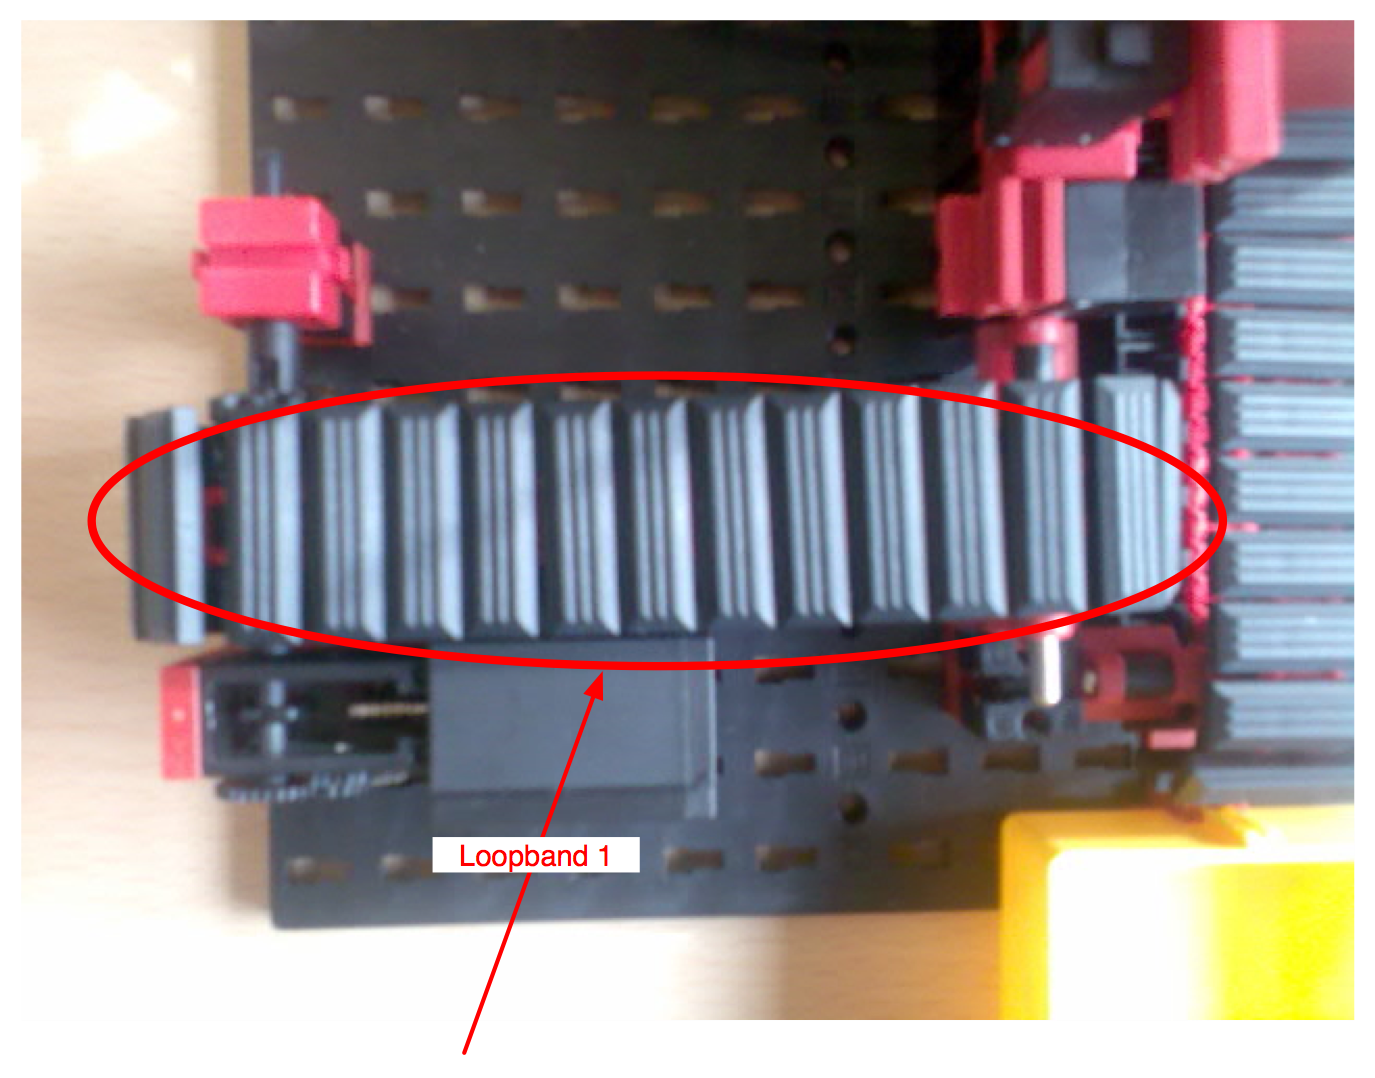
\includegraphics[width=13cm, height=14cm]{LB1} \\

  Dit is de lopende band die de wafers aanlevert. Deze kan alleen vooruit lopen. \\
  Het grote blok ten hoogte van het midden van de band is de motor die deze loopband aandrijft.
% subsection lopende_band_vooruit_ (end)

\subsection{Lopende band (vooruit)}\label{sub:lopende_band_vooruit_} % (fold)
  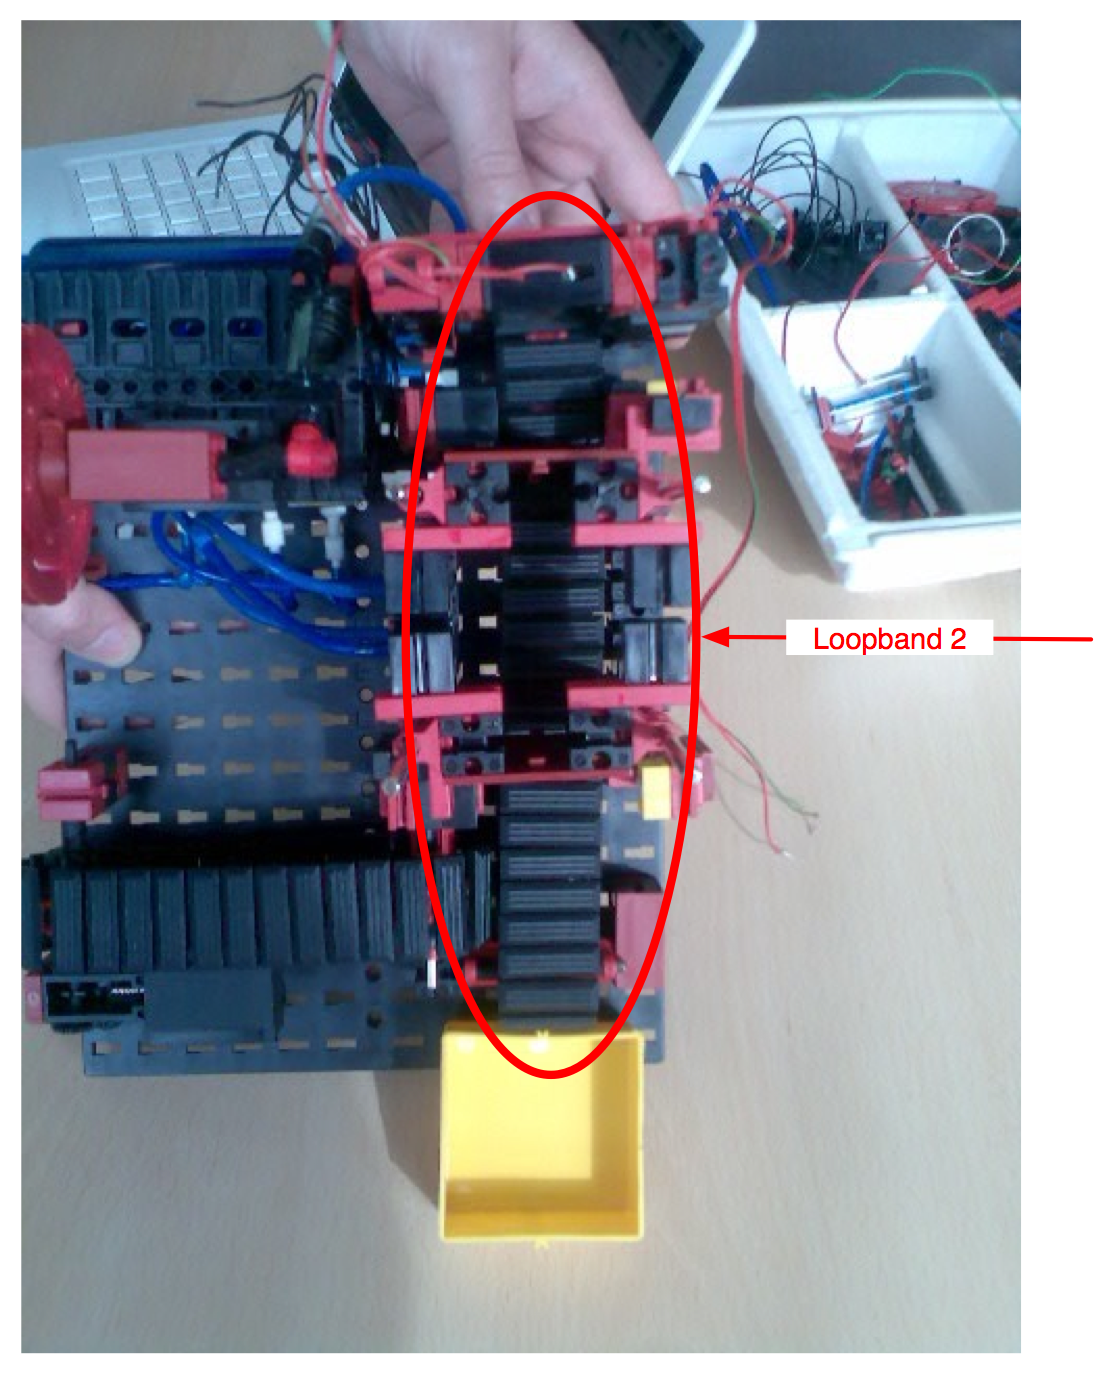
\includegraphics[width=13cm, height=14cm]{LB2} \\

  Dit is de lopende band die de wafers door de twee poorten brengt. Deze band kan voor- en achteruit. \\
   De motor die deze loopband aandrijft is meegenomen in de structuur van het model. Deze maakt deel uit van de pilaar waar de UV-lamp op hangt. Hierdoor hebben wij geen duidelijke foto kunnen maken van de aandrijfmotor.
% subsection lopende_band_vooruit_ (end)

\subsection{Knoppen}\label{sub:knop} % (fold)
  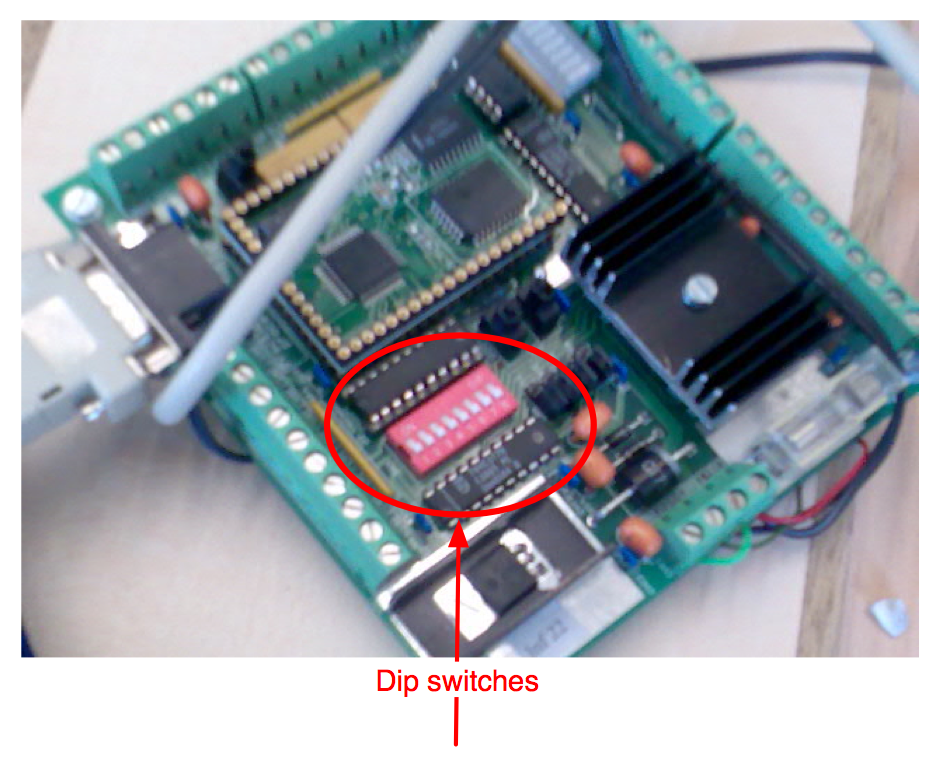
\includegraphics[width=13cm, height=14cm]{dip} \\
  Wij maken gebruik van een DIP-switch, op het geleverde processor bord, als
  startknop. Als noodknop hebben we een aparte knop maar hier is
  geen foto van.
% subsection knop (end)

\subsection{Deur}\label{sub:deur} % (fold)
  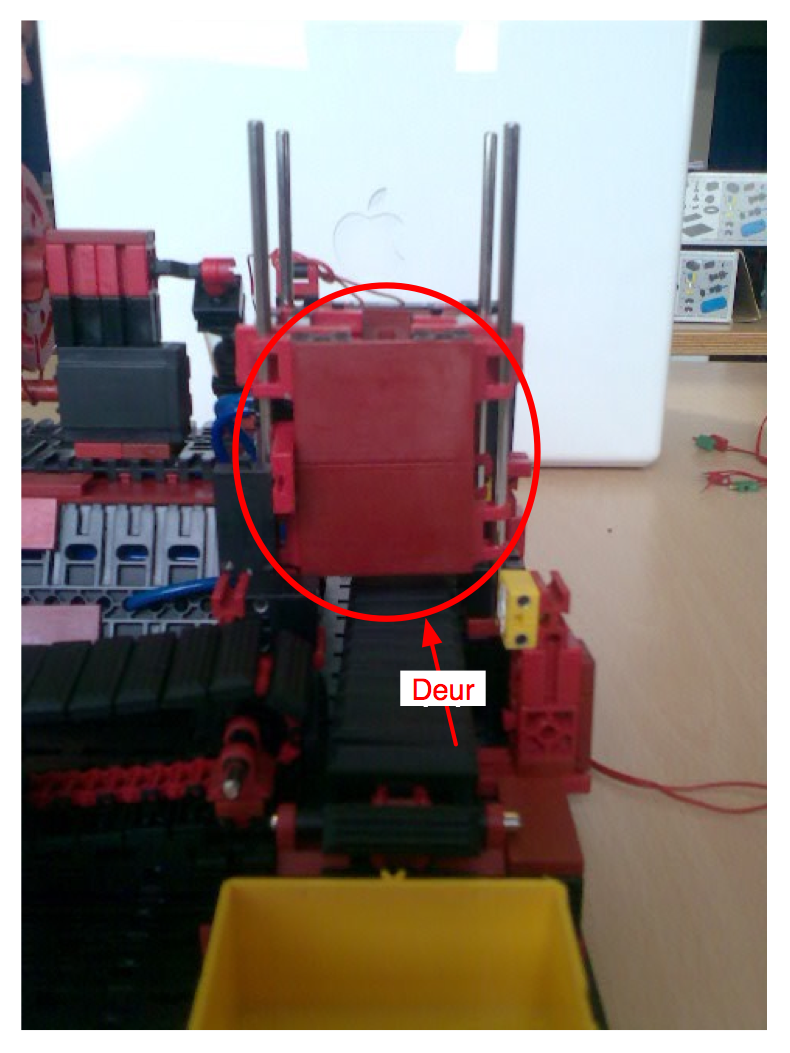
\includegraphics[width=13cm, height=14cm]{deuren_voor} \\
  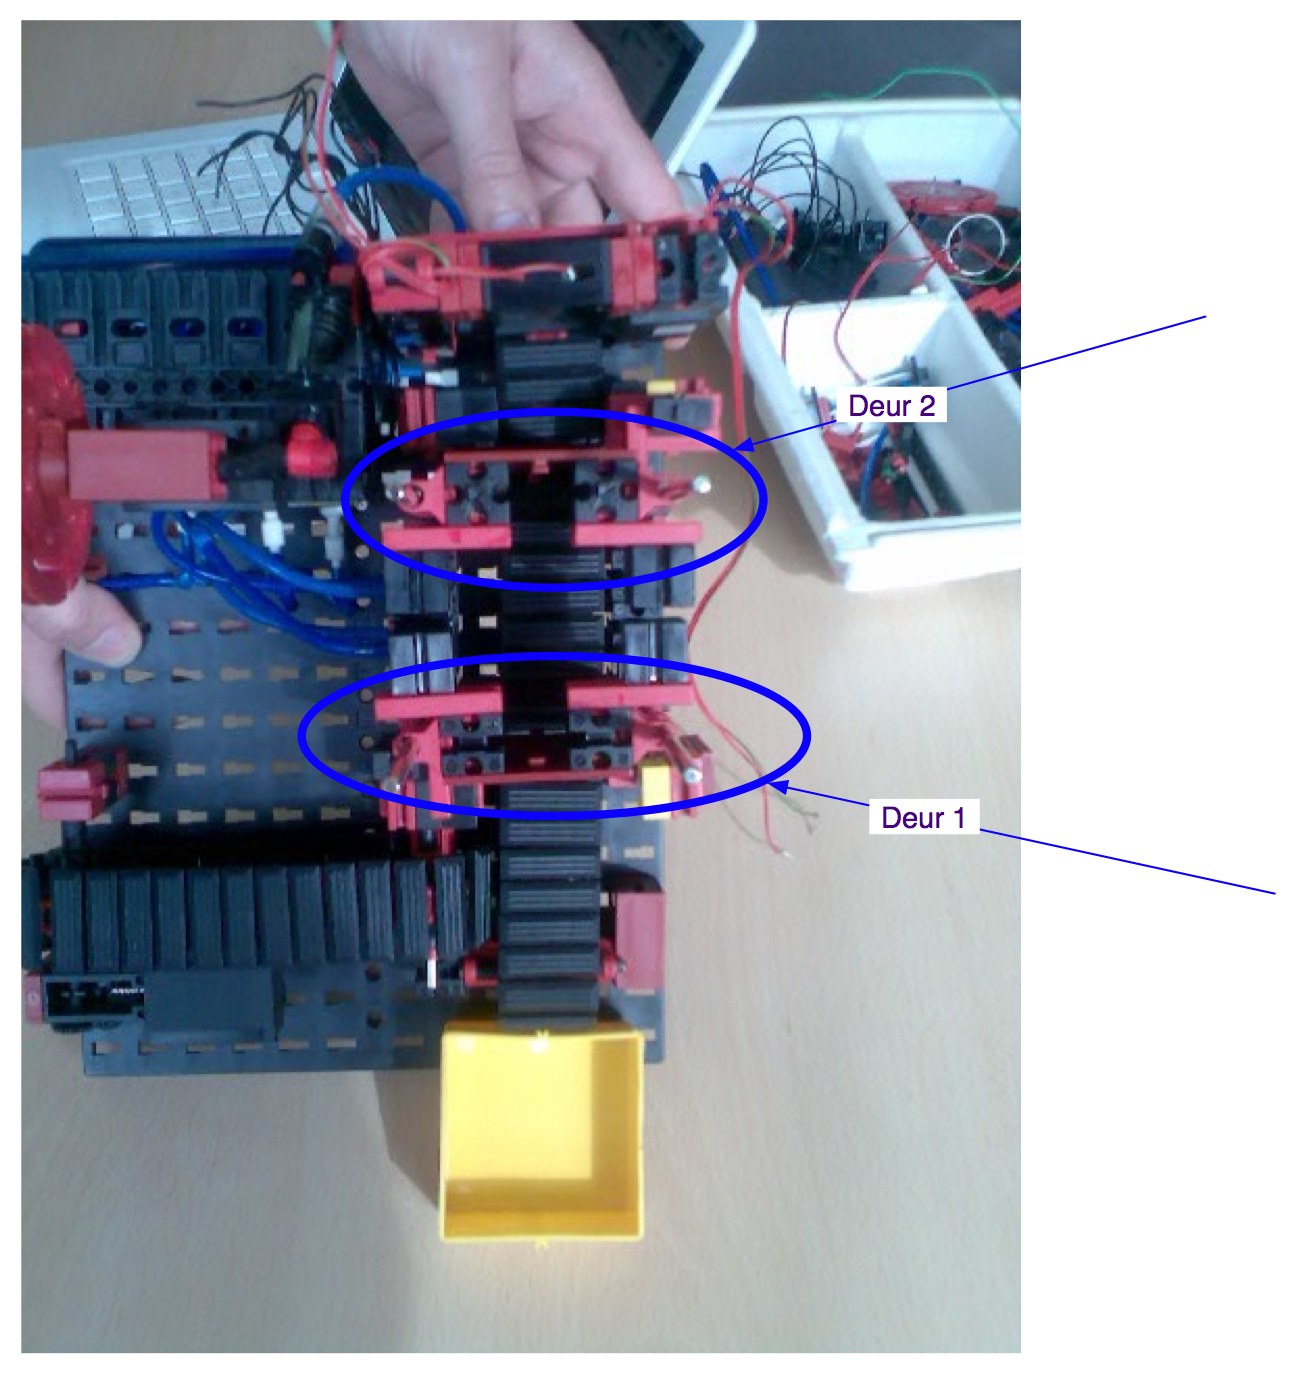
\includegraphics[width=13cm, height=14cm]{deuren} \\

Een voor en boven aanzicht van de twee deuren die de UV-lamp van de
buitenwereld scheiden, zodat deze niet beschadigd kan worden. Wegen
obstructie is er geen vooraanzicht foto van de tweede deur.

% subsection deur (end)


\subsection{Luchtkleppen}\label{sub:luchtkleppen} % (fold)
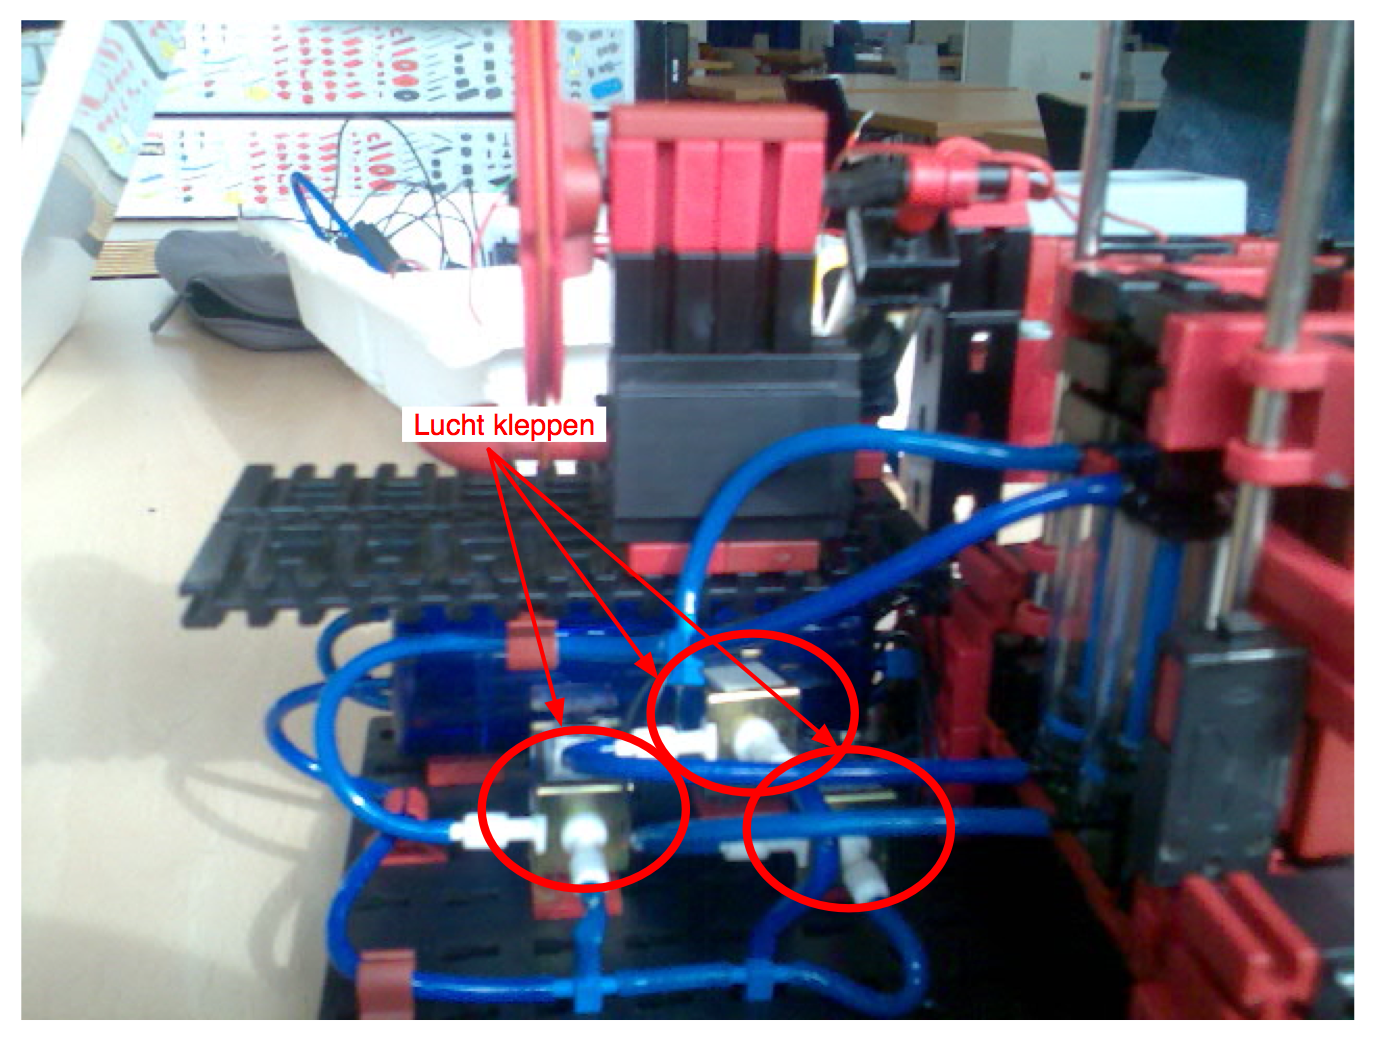
\includegraphics[width=13cm, height=14cm]{valve} \\
Drie van de vier luchtkleppen die gebruikt worden om lucht wel of niet door te laten. De vierde luchtklep is na het maken van deze foto geplaatst, bij de andere drie. Er is hier geen afbeelding van.

% subsection luchtkleppen (end)

\subsection{Compressor}\label{sub:compressor} % (fold)

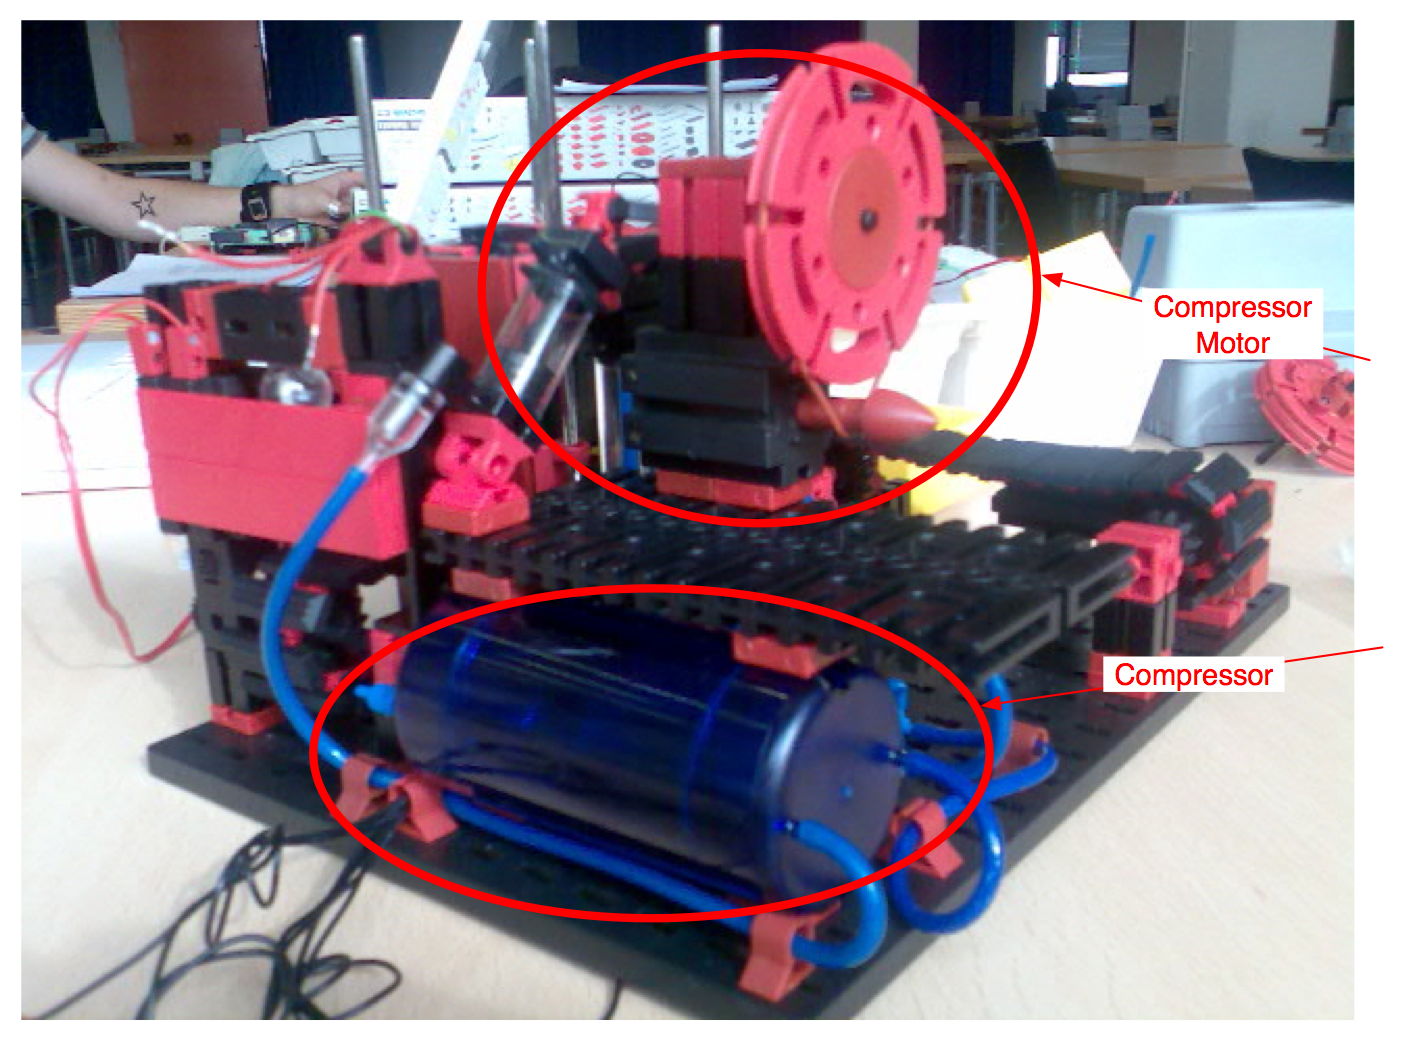
\includegraphics[width=13cm, height=14cm]{compressor} \\
De compressor en de motor die de compressor vult. Deze begint met
draaien zodra het model ingeplugd wordt op het net-stroom. De
compressor en diens motor draaien geheel onafhankelijk van alle
andere onderdelen en kunnen niet worden be\"invloed door de
processor.

% subsection compressor (end)



\subsection{Pnematische Cilinder}\label{sub:pnematische_cilinder} % (fold)

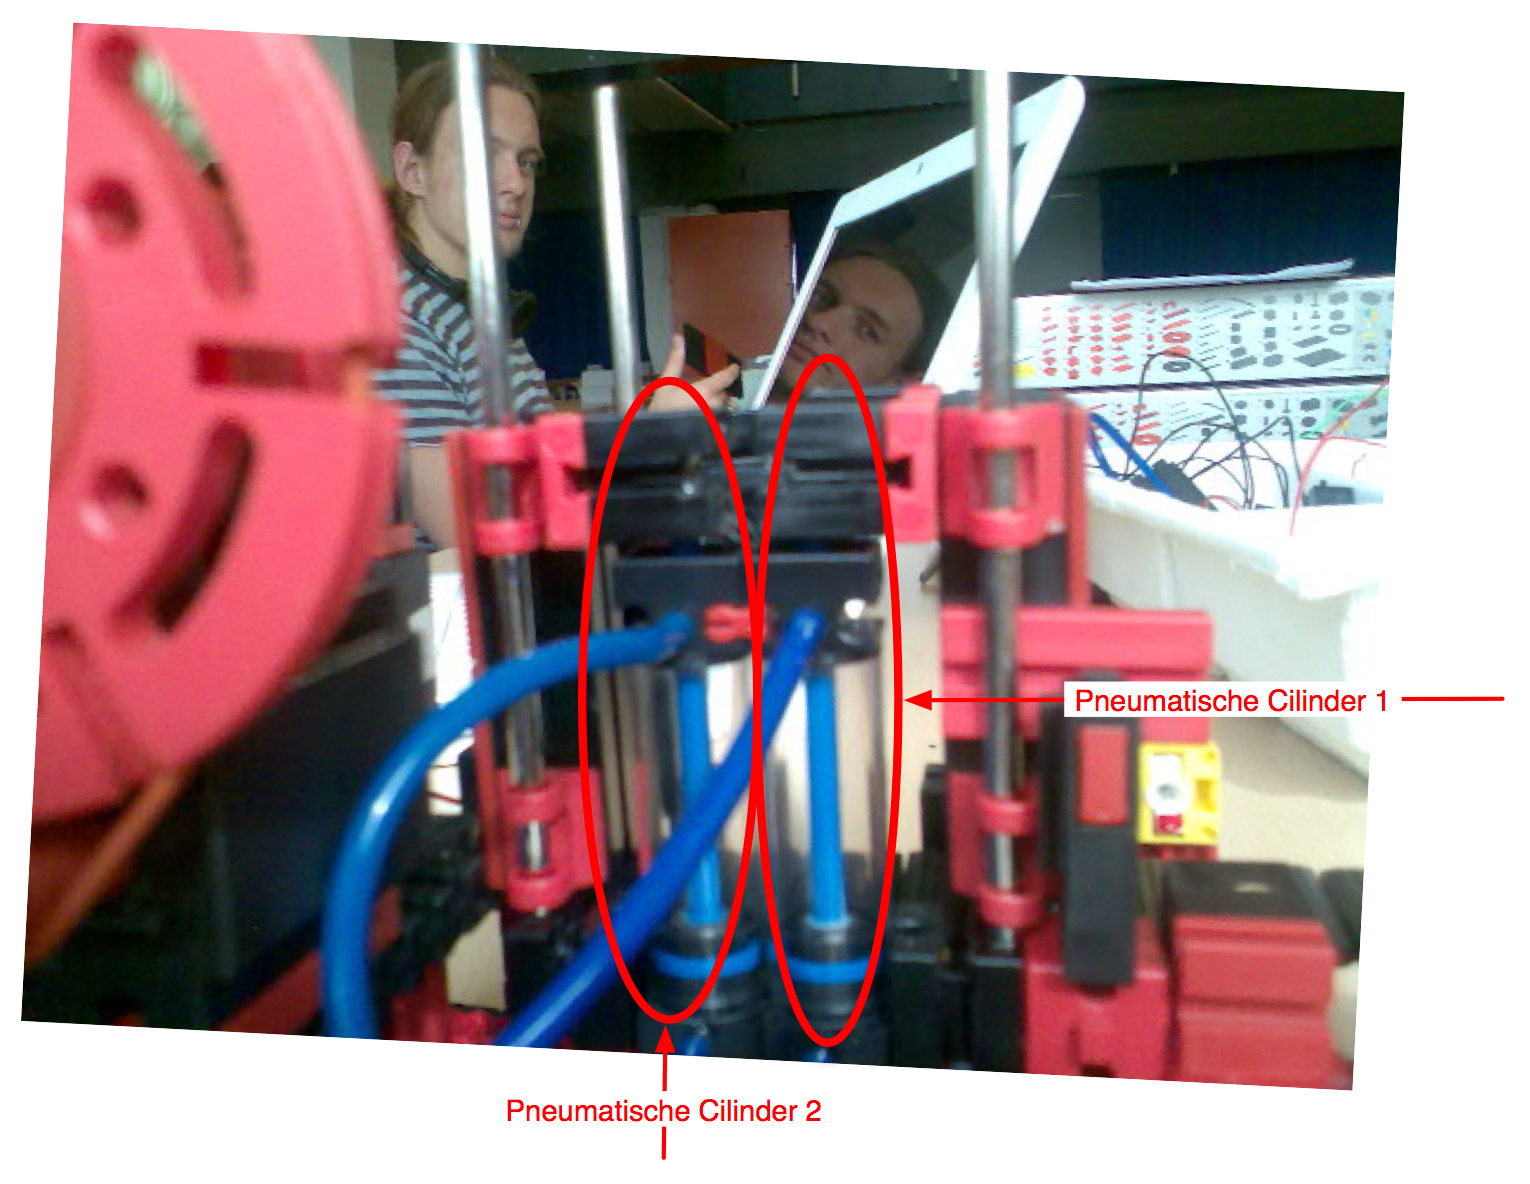
\includegraphics[width=15cm, height=11cm]{PC} \\
De pneumatische cilinder duwt de deur omhoog en trekt hem ook weer omlaag. Wij maken gebruik van twee cilinders, ieder voor \'e\'en deur. De cilinders worden door de luchtkleppen aangestuurd en zijn daarom niet in het UPPAAL model opgenomen.

% subsection pnematische_cilinder (end)

\subsection{Bak}\label{sub:bak} % (fold)

\includegraphics[width=13cm, height=14cm]{lamp} \\
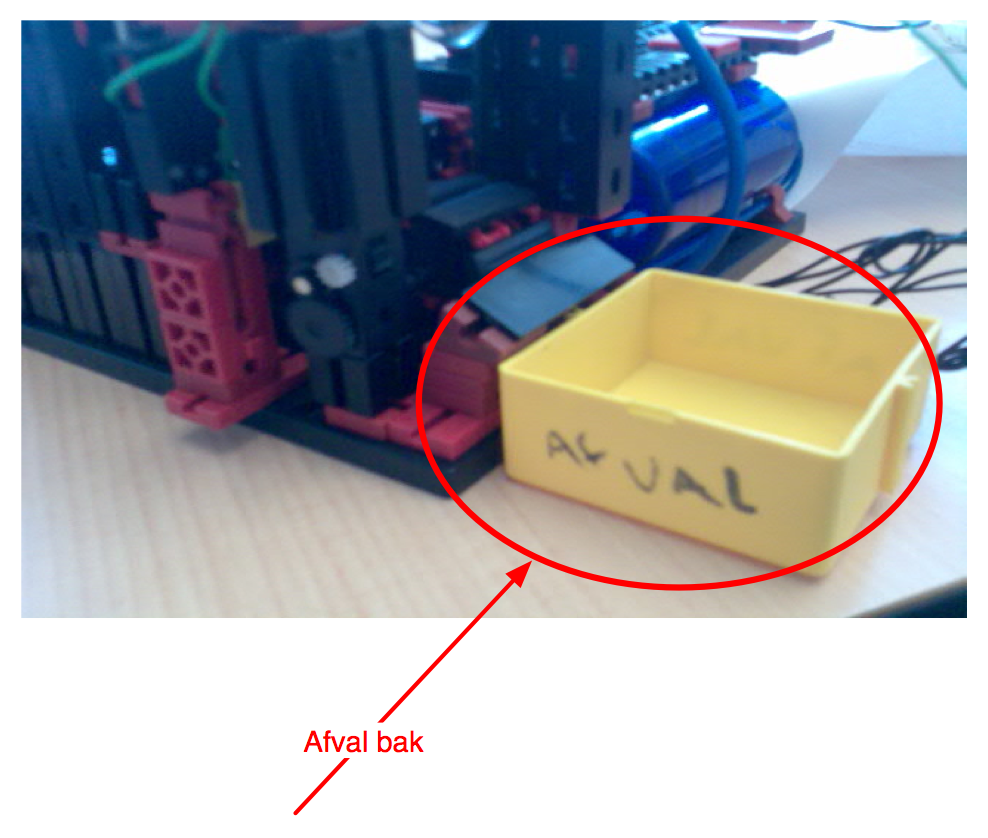
\includegraphics[width=13cm, height=11cm]{afval} \\

De twee bakken voor de gelukte wafers en de afval bak. De afval bak
staat het dichtst bij de UV-lamp. De bak voor de gelukte wafers
staat ver weg van de UV-lamp, voorbij de twee deuren en ter hoogte
van waar de volgende wafer wordt aangeleverd.

% subsection bak (end)

% section foto_s_van_het_model (end)
\section{Ontwerpbeslissingen}
Wij maken gebruik van twee fysieke deuren, die helemaal dicht zijn
en voorkomen dat er een wafer voorbij onze deur komt.
Onze deur wordt omhoog geduwd door 1 cilinder per deur. Dit leek ons het meest logische, een deur die van boven af wordt bestuurd houdt in dat je de luchtkleppen zou moeten inverteren (dicht is dan de valve aan zetten). Een tweede cilinder om de deur omhoog te duwen werkt niet, onze compressor kan daar niet genoeg druk voor opbouwen. Daarom maken wij gebruik van stalen staafjes waar de deuren makkelijk over glijden. \\ \\

Wij hebben besloten om een wafer die mislukt is (omdat er tijdens het bestralen op de noodknop is gedrukt) in een andere bak te deponeren, de afval bak. Hoewel het makkelijker is om de wafer te behandelen als een normale wafer, is het logischer om deze wafers apart te houden, ze zijn immers onbruikbaar. \\ \\

Wij hebben ervoor gekozen om beiden deuren apart aan te sturen. Het is namelijk mogelijk om \'e\'en luchtklep aan te sluiten aan beide deuren, zodat deze beiden tegelijkertijd sluiten. Omwille van mogelijk onderhoud dat gepleegd zou kunnen worden bij een echte wafer stepper, hebben wij ervoor gekozen omdat beiden deur onafhankelijk van elkaar aan te sturen. \\ \\

Wij maken gebruik van twee druksensoren om te kijken of deur dicht is. Hoewel aangekondigd was dat er niet genoeg druksensoren waren om beiden deuren te controleren, hadden wij in onze dozen twee druksensoren. De zijn beiden gekoppeld aan de onderkant van de deur. Beiden deuren hebben een uitsteekseltje om de druksensor te activeren indien de deur dicht is. \\ \\




\chapter{UPPAAL model}\label{chap:uppaal_model} % (fold)


% section uppaal_model (end)

Dit zijn al onze UPPAAL componenten. \textit{Opmerking:} deze
versies van ProgramInit en ProgramRun zijn verouderd. Hierdoor
kloppen een paar dingen niet meer. Zo waren bPress[1] en bRelease[1]
eerst kanalen die aangaven dat de noodknop ingedrukt respectievelijk
losgelaten werd, maar zijn er nu een nieuwe noodknop-template en
daardoor (handigere) emStart en emStop kanalen. Zie voor een goede
versie van het hoofdprogramma het programmaontwerp.

\begin{itemize}
    \item ``ProgramInit'' wordt aan het begin van het programma uitgevoerd. Dit zorgt ervoor dat alle actoren in een wenselijke toestand zijn. Als ProgramInit klaar is, wordt ProgramRun aangeroepen. \textit{Opmerking:} we mogen
    er van uit gaan dat alles in het begin in de wenselijke toestand is, dit hebben we in het programmaontwerp dan ook gedaan, waardoor daar geen ProgramInit of equivalent daarvan te vinden is. \\
    \textbf{Program Init} \\
    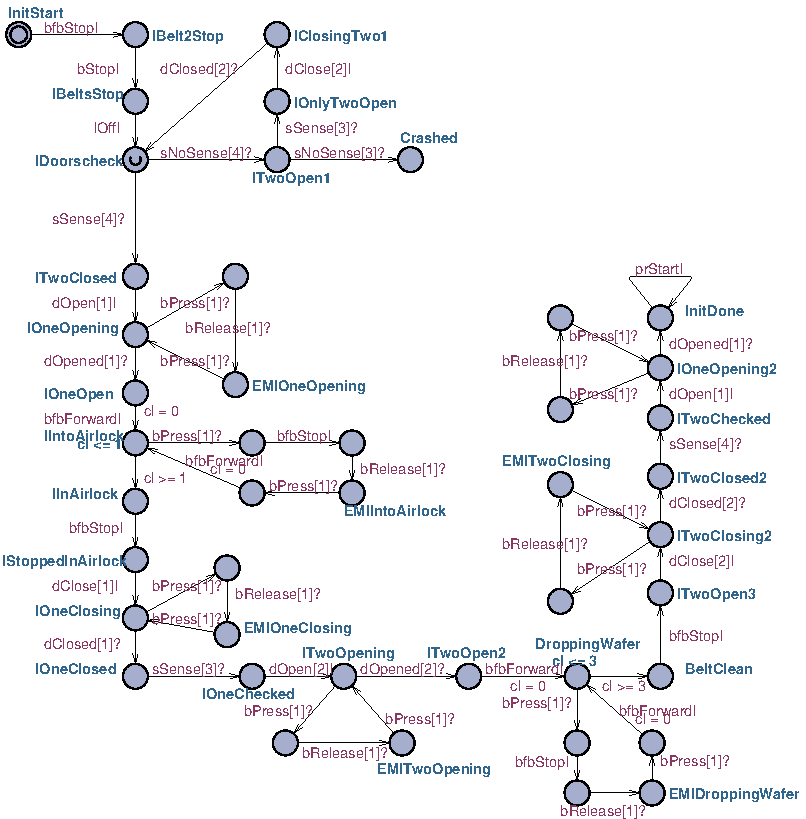
\includegraphics[scale=.7]{ProgramInit} \\
    \textbf{Program Run} \\
    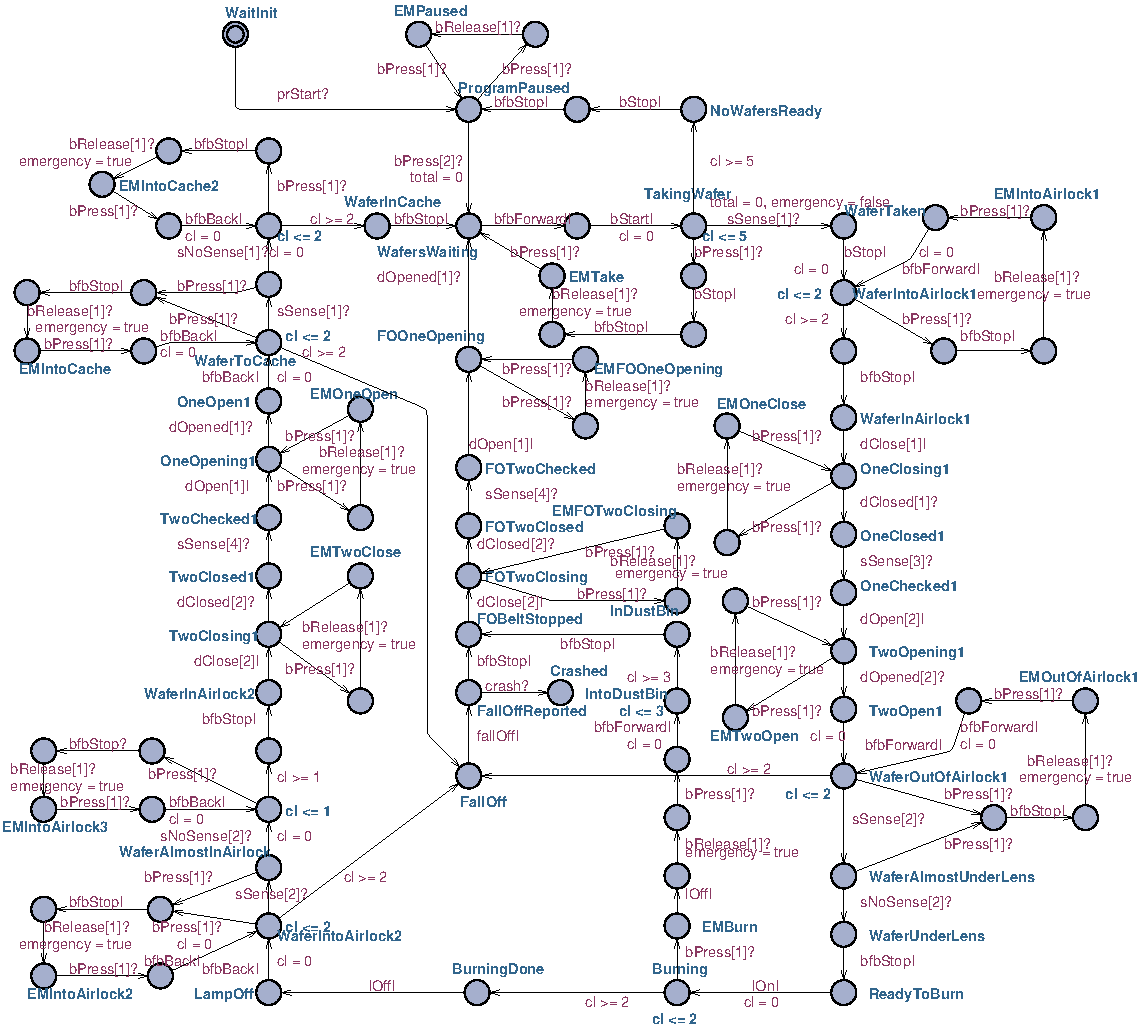
\includegraphics[scale=.7]{ProgramRun} \\
    \item ``StartButton'' staat voor de startknop. Deze kan alleen ingedrukt worden, er wordt dan een signaal verstuurd waardoor het systeem start.  \\
    \textbf{StartButton} \\
    
\includegraphics{UPstartbutton} \\
    \item ``EMButton'' staat voor de noodknop. Hier zijn drie toestanden mogelijk. E\'{e}n toestand stelt een emergency voor, \'{e}\'{e}n
    toestand wordt bereikt als het systeem uit een emergency komt en de laatste toestand zorgt ervoor dat het systeem niet gelijk weer in emergency
    kan gaan als een emergency afgelopen is. \\
    \textbf{EMButton} \\
    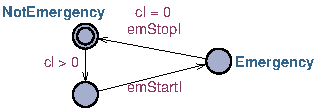
\includegraphics{UPEMbutton} \\
    \item ``Lamp'' staat voor een LED of de UV-lamp. Deze kan aan of uit staan. \\
    \textbf{Lamp} \\
    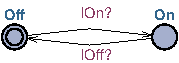
\includegraphics{UPlamp} \\
    \item ``Conveyor'' is de lopende band die maar 1 kant op kan lopen. Deze kan dus 'aan' (running) of 'uit' (stopped) zijn.\\
    \textbf{Conveyor} \\
    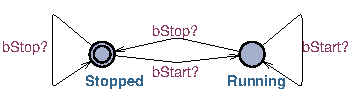
\includegraphics{UPconveyor} \\

    \item ``ConveyorBF'' kan heen en terug lopen. Er zijn dus toestanden voor back, forward en stopped nodig.\\
    \textbf{ConveyorBF} \\
    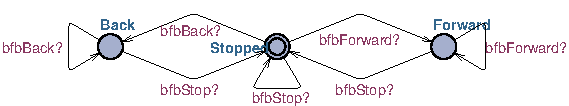
\includegraphics{UPconveyorBF} \\
    \item ``Door'' is het model van een deur. Een deur kan open of dicht zijn. Als een geopende deur een open-signaal krijgt (of een gesloten deur een sluit-signaal), dan wordt dit verwerkt door meteen aan te geven dat de deur klaar is met openen (of sluiten).\\

    \textbf{Door} \\
    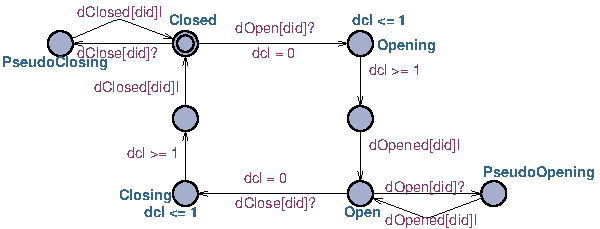
\includegraphics{UPdoor} \\
    \item ``Sensor'' is een licht- of druksensor. Een sensor kan Sense of NoSense zijn - hij neemt iets waar of hij neemt niets waar.\\
    \textbf{Sensor} \\
    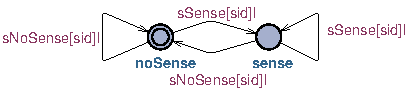
\includegraphics{UPsensor} \\
    \item ``FallOff'' - dit is een speciaal geval. Het is niet echt een hardware-component (ondanks dat er wel LEDs aan en uit gaan ten gevolge van de toestand van dit onderdeel). FallOff houdt bij hoeveel wafers van de band gevallen zijn. Zodra er vijf wafers verloren zijn gegaan 'crasht' ons systeem (dit is een noodtoestand). We houden dit op deze manier bij omdat de hoeveelheid verloren wafers van groot belang is voor de werking van het systeem.\\
    \textbf{falloff} \\
    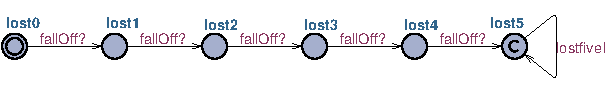
\includegraphics{UPfalloff} \\
\end{itemize}

Veel van de componenten hebben een onbekende beginstand, een gegeven dat gemodelleerd is door vanuit Init een stap te maken naar een willekeurige toestand.\\
Daarnaast wordt van veel componenten verwacht dat ze een signaal kunnen versturen,  (``deze deur staat open!'') - dit wordt gedaan door in elke  'stabiele' toestand (de deur staat open) een loopje naar dezelfde toestand te maken. Deze loop verstuurt een signaal over het gewenste kanaal.



\section{Ontwerp Beslissingen}\label{sec:ontwerp_beslissingen} % (fold)

We hebben expliciet gekozen om geen wafer-element toe te voegen. Dit
zou namelijk betekenen dat de wafers zelf te besturen zijn, iets dat
niet zo is. Er is helemaal niets bekend over de wafer, alleen over
het feit dat sensoren iets registreren of niet. Uit deze informatie
kan dan weer worden afgeleid waar een wafer is.\\ \\

``FallOff'' is expliciet gedeclareerd omdat er bepaalde lampjes zijn
die overeenkomen met een aantal wafers die weg zijn. Elke toestand van
``FallOff'' bestuurd nu impliciet die lampjes. Daarnaast is het zo dat
zodra de vijfde wafer van de band af valt er een noodstop gemaakt
moet worden. \\ \\


% chapter ontwerp_beslissingen (end)










%Al deze onderdelen spreken voor zich, behalve de Teller. Dit element
%houdt bij hoeveel wafers er van de band afgevallen zijn. De
%onderdelen hebben hun eigen template en mogelijkheden om te
%communiceren met de buitenwereld. Hierdoor kunnen orders gegeven
%worden aan actoren en de staat van sensoren gelezen worden.
%
%
%\section{Ontwerpbeslissingen}
%

%
